\documentclass[10pts,fleqn]{article}

\usepackage{url}
\usepackage{mydefs}
\usepackage{notes}
\usepackage{graphicx}
\usepackage{algorithm,algorithmic}

\newenvironment{packeditemize}{
\begin{itemize}
  \setlength{\itemsep}{1pt}
  \setlength{\parskip}{-2pt}
  \setlength{\parsep}{-2pt}
}{\end{itemize}}

\newenvironment{packeddescription}{
\begin{description}
  \setlength{\itemsep}{1pt}
  \setlength{\parskip}{0pt}
  \setlength{\parsep}{0pt}
}{\end{description}}

\newenvironment{packedenumerate}{
\begin{enumerate}
  \setlength{\itemsep}{1pt}
  \setlength{\parskip}{0pt}
  \setlength{\parsep}{0pt}
}{\end{enumerate}}


\title{Multiple Task Learning for Very Many Tasks in Very Many Dimensions}

\begin {document}

\maketitle

\begin{abstract}
\end{abstract}



%=============================================================================================================
\section{Introduction}

{\bf Goal:} Perform multitask learing for millions of tasks in very high dimensions.

%\begin{packeditemize}
\begin{itemize}
	\item consider a matrix $M \in \mathbb{R}^{TxD}$ with the rows as $T$ task and the columns are $D$ features or dimensions. Now the $T$ is really big and so we need to cluster the tasks. Also, the dimension $D$ is very large and we need to cluster the dimensions too. So it seems like we are clustering on the rows and columns of matrix $M$. Hence, in this case we treat the multitask learning as a co-clustering problem.
	\item an alternate way to achieve the above is by viewing the problem as a matrix decomposition problem where we have $M = ABC$ and $A \in \mathbb{R}^{TxT'}$, $B \in \mathbb{R}^{T'xD'}$ and $C \in \mathbb{R}^{D'xD}$. Consider $T'$ as the clustered super tasks and the $D'$ as the clustered super-words. The matrix $B$ that relates the task-clusters with the word-clusters is infact our relationship matrix here. In case of large number of dimensions as well as large number of features it is infeasible to work with the resulting matrix and the hope here is that a a reduced dimensional or low rank representation on both the rows and columns will make the learning process myuch more tractable.
	\item we assume the super-task and the super-word structure to be latent variables and model them using LDA. Both the super-task and super-word can learned alternately and also be used to update each other. Also, note that in the above the clustering on row-space is supervised whereas the clustering on the column space is unsupervised.
\end{itemize}
%\end{packeditemize}



%=============================================================================================================
\section{Generative Model}

\begin{enumerate}
	\item row-clustering
	\begin{enumerate}
		\item each task is drawn from a distribution of super-doc
		\item each super-doc is drawn from a distribution of docs
	\end{enumerate}
	\item col-clustering
	\begin{enumerate}
		\item each doc is drawn from a distribution of super-words (topics)
		\item each super-word (topic) is drawn from a distribution of words
	\end{enumerate}
\end{enumerate}
NOTE: the above two apparently disconnected clustering steps are linked by step 1(b) and 2(a).

In any large scale application, the number of data points as well as the feature
dimension are both extremely large. For example, we can consider a corpus of
text documents where the number of documents is huge and the size of the vocabulary is
of the order of several tens of thousands. Additionally, the documents might belong
to some groups. Such groups can be discovered in a completely unsupervised fashion
or there might also be partial supervision available for some of these groups.

We start with a document by words matrix. The idea here is to decompose this matrix as a product of
three matrices -- documents by tasks, tasks by topics and topics by words. In the
first matrix, the documents are categorized into some tasks or groups.
Documents in each task are assumed to have a distinctive
distribution in the topic space, as dictated by the second matrix.
The third matrix denotes the structure of the topics.
In a typical topic model framework, the document by words matrix is
decomposed as a product of two matrices -- document by topics and topic by words.
Here, we go one extra level up and try to discover the document groups
either in a completely unsupervised way or using limited amount of supervision.

One could solve the problem of document clustering into multiple
tasks and the topic modeling in a separate framework. Since topic models project documents
onto topic space, one could work with the topic space representation of the documents
and group documents using the topic space assignment
in a post-processing step. However, as exemplified in a recent research
\cite{xixi13}, incorporating information about documents' latent
groups further improves the performance of topic models and the assignment
of the documents into latent groups can be bettered from this
revised topic model.
Our objective is to follow this research direction and propose methods for
large scale distributed inference techniques and extend the models to non-parametric
setting where the number of groups can be inferred from the data itself.
The online inference techniques used in topic model are essentially
stochastic gradient descent applied to variational EM framework
\cite{hobb10,wapb11}. For large scale applications, online variational
inference has been shown to be successful. We, therefore, plan to use such
framework for large scale non-parametric multitask learning.

Much of the large scale data available in industry reside in different
machines and necessitates distributed processing instead
of aggregating all the data in the same place. One particular scenario
is when the features of the data lie in different physical locations. For example, the data for
Yahoo! mail and Yahoo! news for the same user reside in different
cluster machines. We plan to propose techniques for distributed online variational inference
using alternating direction method of multipliers (ADMM)\cite{bopc11}.


%=============================================================================================================
\section{Last discussion}
\begin{figure}[!htbp]
	\centering
	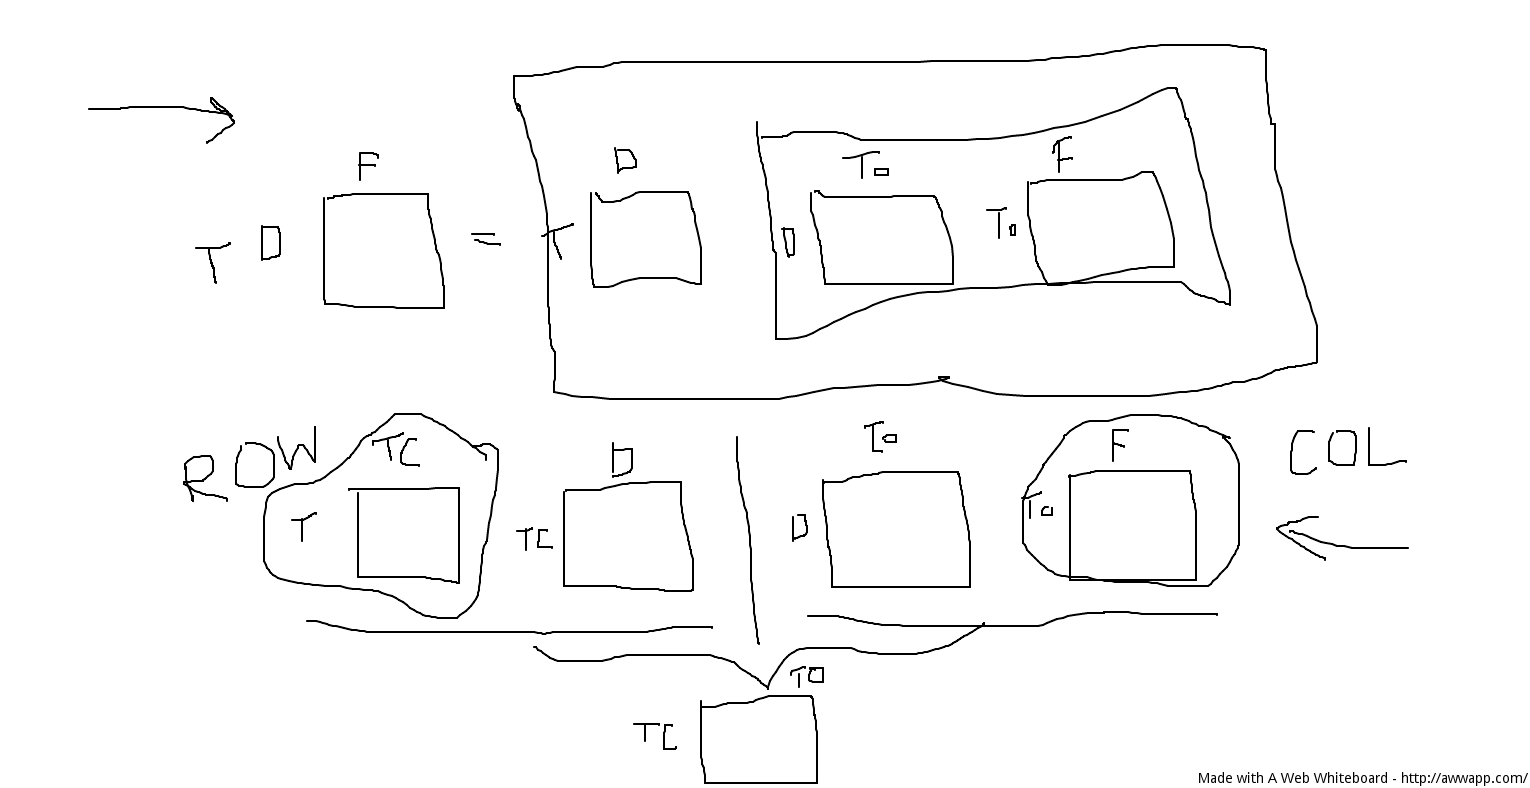
\includegraphics[width=1.05\textwidth]{50.png}
	\caption{Our last discussion}
\end{figure}

%=============================================================================================================
\bibliographystyle{plain}
\bibliography{refs,latestbib}

\end {document} 
